\documentclass[11pt]{beamer}
\usefonttheme[onlymath]{serif}
\usepackage[utf8]{inputenc}
\usepackage[T1]{fontenc}
\usepackage{bbm}
\usepackage{lmodern}
\usepackage{amsthm}
%\usepackage[francais]{babel}
% \usepackage[hidelinks]{hyperref}
\usepackage[autolanguage]{numprint}
\usepackage[utf8]{inputenc}
\usepackage[T1]{fontenc}
\usepackage{icomma}
\usepackage{fancybox}
\usepackage{tikzsymbols}
\usepackage{MnSymbol,wasysym}
\newtheorem{rem}{Remarque}
\newtheorem{deff}{Définition}
\newtheorem{lem}{Lemme}
\newtheorem{prop}{Proposition}
\newtheorem{propr}{Propriété}
\newtheorem{ex}{Exemple}
\newtheorem*{ex*}{Exemple}
\newtheorem{algo}{Algorithme}
\newtheorem*{algo*}{Algorithme}
\newtheorem{theoreme}{Théorème}
\newtheorem*{preuve*}{Preuve}
\newtheorem{preuve}{Preuve}

\newtheorem{acknowledgement}[theorem]{Remerciements}
\newtheorem{algorithm}[theorem]{Algorithme}
\newtheorem{axiom}[theorem]{Axiom}
\newtheorem{case}[theorem]{Case}
\newtheorem{claim}[theorem]{Propriété}
\newtheorem{conclusion}[theorem]{Conclusion}
\newtheorem{condition}[theorem]{Condition}
\newtheorem{conjecture}[theorem]{Conjecture}

\newtheorem{criterion}[theorem]{Criterion}


\newtheorem{exercise}[theorem]{Exercice}

\newtheorem{notation}[theorem]{Notation}

\newtheorem{proposition}[theorem]{Proposition}
\newtheorem{remark}[theorem]{Remarque}

\newtheorem{summary}[theorem]{Résumé}
\newcounter{saveenumi}
\newcommand{\seti}{\setcounter{saveenumi}{\value{enumi}}}
\newcommand{\conti}{\setcounter{enumi}{\value{saveenumi}}}
\usepackage{tikz-qtree}
\usepackage{tikz}
\usepackage{scalerel,stackengine}
\usepackage{subfig}
\usepackage{forest}
\usepackage{smartdiagram}
\usesmartdiagramlibrary{additions}

% \usepackage{vietnam}
\usepackage{varwidth}
%\usepackage[figurename=Illustration]{caption}
%\usepackage[francais]{babel}

\smartdiagramset{module minimum width=3cm, module minimum height=2cm, text width=8em, font=\small, circular distance = 5cm}

% Tikz options --------------------------------------------
\usetikzlibrary{arrows,shapes,positioning,shadows,trees}
\tikzset{
  basic/.style  = {draw,  drop shadow, font=Helvetica, rectangle, align=flush center},
  root/.style   = {basic, rounded corners=2pt, thin, align=flush center, fill=blue!30, text width=13em},
  level 2/.style = {basic, rounded corners=8pt, align=flush center, fill=blue!20, text width=8em, minimum height=30pt},
  level 3/.style = {basic,  align=flush left, fill=orange!10, text width=9em, rounded corners = 4pt}
}
%---------------------------------------------------------

%\frenchbsetup{CompactItemize=false}

% \usepackage[babel]{csquotes}
% \usepackage[url=false, doi=false, style=science, backend=bibtex, bibencoding=ascii]{biblatex}
% \bibliography{IEEEabrv,bib/OAM}

\usepackage{tikz}
\usepackage{pdfrender}

\usetikzlibrary{shapes,arrows}
%\setbeamerfont{author}{size=\Huge}
%\setbeamerfont{institute}{size=\normalsize\itshape}
%\setbeamerfont{title}{size=\fontsize{30}{36}\bfseries}
%\setbeamerfont{subtitle}{size=\Large\normalfont\slshape}

\hypersetup{
  colorlinks=true,
  citecolor=blue,
  linkcolor=black,
  filecolor=magenta,
  urlcolor=cyan,
}

\mode<presentation> {
  %\useoutertheme{infolines} % Pour les thèmes qui n'ont pas de pied-de-page
  \usetheme{ulaval}
  %\usecolortheme{ulaval}
  % \setbeamercovered{transparent}
  \setbeamercovered{invisible}
  %\setbeamertemplate{navigation symbols}{} % Enlever les icônes de navigation
}


%\usepackage{bm}
% For typesetting bold math (not \mathbold)
%\includeonlyframes{}

%\usepackage{pgfpages}
%\setbeameroption{show notes on second screen}
%\setbeameroption{show notes}
%\setbeamertemplate{note page}[plain]

\logo{%\includegraphics[height=0.6cm]{COPL}\hspace{.5cm}%

\includegraphics[height=0.5cm]{UL_P}}%\hspace{.2cm}\vspace{.865\paperheight}}
\titlegraphic{
\includegraphics[height=1.5cm]{UL_actu}}


\title[]{État de l'avancement des travaux}
\subtitle[]{Projet de recherche été 2019}

\author[Lepage A., N'Diaye D. et Zito A.]{Alexandre Lepage, Diamilatou N'Diaye \newline et Amedeo Zito}
\institute[ULaval] % École d'actuariat
{
  École d'actuariat \\
  Université Laval, Québec, Canada \\
}

\date{2019-05-31} % \today will show current date.
%\today
% Alternatively, you can specify a date.
% \today


\AtBeginSection[]{
\begin{frame} 
	\Huge\centerline{\insertsection}
	%  \small \tableofcontents[currentsection, hideothersubsections]
\end{frame}
}

\setbeamertemplate{theorems}[numbered]

%\AtBeginSection[]
%  {
%     \begin{frame} <beamer>
%     \frametitle{Agenda}
%     \tableofcontents[currentsection]
%     \end{frame}
%  }
%  
\newenvironment{slide}[1]
{\begin{frame}[environment=slide]
\frametitle{\insertsection \newline \large{#1}}}
{\end{frame}}

\begin{document}

\begin{frame}[label=titre, plain]
\titlepage
\end{frame}


\section{Revue de littérature}
\subsection{Itre 4}
\begin{frame}
	\frametitle{Revue de littérature}
	\framesubtitle{Itre4: Hierarchical Archimedean copulas through multivariate compound
		distributions \cite{Itre4}}
	
	\textbf{Copule archimédienne}
	
	\begin{itemize}
		\item Soit $\Theta_i = \sum_{j=1}^{M} B_{i,j}$, où $M$ et $\underline{B}$ sont indépendants et les $B_{i,j}$ sont i.i.d. pour un même $i$.
		\begin{figure}[H]
			\centering
			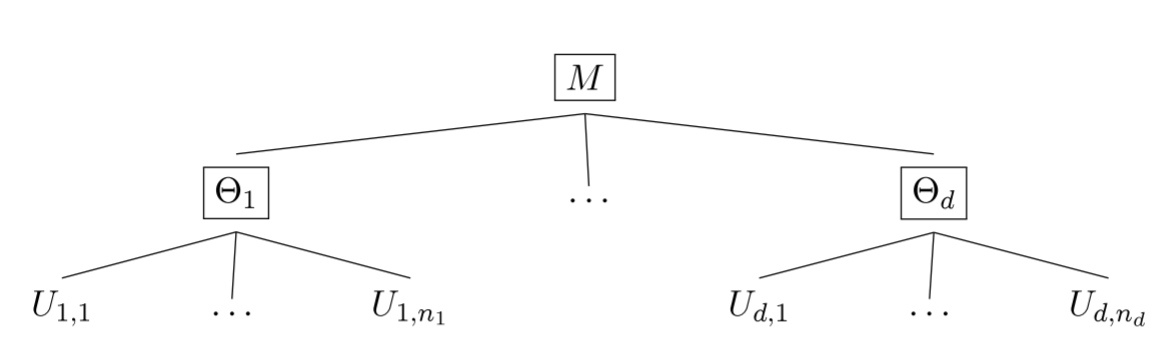
\includegraphics[height=3cm]{Hierarchie_1}
			\renewcommand{\figurename}{Illustration}
			\caption{Arbre hiérarchique à un niveau.}\label{hierarchie}
		\end{figure}
	
	\end{itemize}
\end{frame}


\begin{frame}
	\frametitle{Revue de littérature}
	\framesubtitle{Itre4: Hierarchical Archimedean copulas through multivariate compound
		distributions \cite{Itre4}}
	\begin{itemize}
		\item Copule archimédienne à un niveau:
		\begin{align}
			C(u1, ... , u_k) 
			&= \mathcal{L}_{\Theta}\left(
				\sum_{i=1}^{k} \mathcal{L}_{\Theta}^{-1} (u_i) \right) \nonumber \\
			&= \mathcal{L}_{M}\left(
				\sum_{i=1}^{d} - \ln \left(
				 \mathcal{L}_{B_i}\left(
				  \sum_{j=1}^{n_i} \mathcal{L}_{\Theta_i} (u_{i,j})
				\right) \right)\right), \label{Copule_Archimedienne}
		\end{align}
		où $d$ correspond au nombre de liens de dépendance différents à modéliser à travers la copule et $\{n_i,\ i=1,...,d\}$ correspond au nombre d'uniformes qui sont générées par groupe de dépendance.
		
	\end{itemize}

\end{frame}


\subsection{Itre 5}
\begin{frame}
	\frametitle{Revue de littérature}
	\framesubtitle{Itre5: Collective Risk Models Dependence \cite{Itre5}}

		\textbf{Le modèle sous-jacent:}
		\begin{itemize}
			\item Soient $N$, la v.a. du nombre de sinistres et $X_k$, la v.a. de la sévérité des sinistres.
			
		\begin{equation}\label{Modele_collectif}
			S = \sum_{k=1}^{N} X_k,
		\end{equation}
		où $N$ est dépendant de $\underline{X}$ et les $X_k$ sont dépendants entre eux.
	
		\end{itemize}
\end{frame}


\begin{frame}
	\frametitle{Revue de littérature}
	\framesubtitle{Itre5: Collective Risk Models Dependence \cite{Itre5}}
	
	\begin{figure}[H]
		\centering
		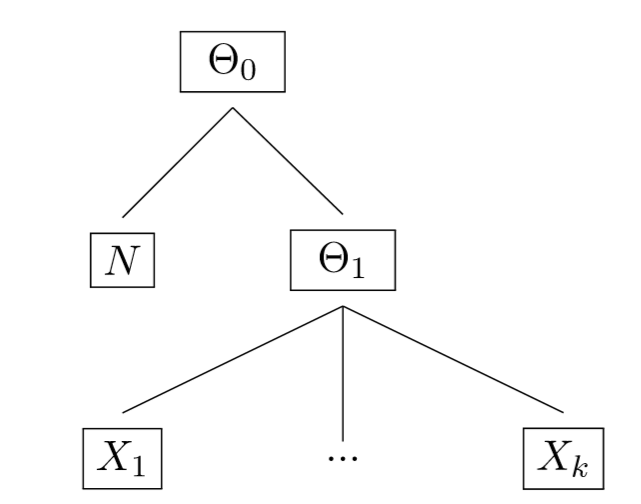
\includegraphics[height=4cm]{Hierarchie}
		\renewcommand{\figurename}{Illustration}
		\caption{Arbre hiérarchique du modèle collectif de risque avec dépendance, où $\Theta_0$ correspond à $M$ et $\Theta_1 = \sum_{i=1}^{M}B_i$, avec les $B_i$ qui sont i.i.d. et indépendants de $M$.}\label{hierarchie_Modele_collectif}
	\end{figure}
	
\end{frame}


\begin{frame}
	\frametitle{Revue de littérature}
	\framesubtitle{Itre5: Collective Risk Models Dependence \cite{Itre5}}
	
	\begin{itemize}
		\item Adaptation de la copule archimédienne hiérarchique dont la formule apparaît en \eqref{Copule_Archimedienne} au modèle collectif définit en \eqref{Modele_collectif}.

		\begin{equation*}
			C(u_0, ..., u_k) = \mathcal{L}_M \left( 
				\mathcal{L}_{M}^{-1} (u_0) - \ln \left(
					\mathcal{L}_B \left(
						\sum_{i=1}^{k} \mathcal{L}_{\Theta_1}^{-1}(u_i)
							\right)\right)\right)
		\end{equation*}
	\end{itemize}
\end{frame}


\begin{frame}
	\frametitle{Revue de littérature}
	\framesubtitle{Itre5: Collective Risk Models Dependence \cite{Itre5}}
	
	\textbf{Méthodes de simulation:}
	\begin{itemize}
		\item avec l'algorithme de Itre 4,
		\item avec la transformation de Fourrier.
	\end{itemize}
	
\end{frame}


\begin{frame}
	\frametitle{Revue de littérature}
	\framesubtitle{Itre5: Collective Risk Models Dependence \cite{Itre5}}
	
	\textbf{Calculs exactes} avec la distribution multivariée de mélange d'Erlang:\\
	
	\begin{itemize}
		\item Soit $V_j$, une v.a. permettant d'introduite la dépendance entre les éléments de $\underline{X}$ de telle sorte que les $(X_i|V=v)$ sont conditionnellement indépendants.
		
		\begin{equation*}
		F_S(x) = Pr(N=0) + \sum_{n=1}^{\infty} \sum_{v=1}^{\infty} \gamma_{N,V}(n,v) H(x; nv, \beta)
		\end{equation*}
		
		\begin{equation*}
		TVaR_{\kappa}(S) = \frac{1}{1-\kappa} \sum_{n=1}^{\infty} \sum_{v=1}^{\infty} \gamma_{N,V}(n,v) \frac{nv}{\beta} \bar{H}(VaR_{\kappa}(S); nv + 1, \beta)
		\end{equation*}
		
	\end{itemize}
\end{frame}


\section{Lectures en cours}
\begin{frame}
	\frametitle{Lectures en cours}
	
	\begin{enumerate}
		\item Everything You Always Wanted to Know about Copula Modeling but Were Afraid to Ask \cite{Everything}
		\newline
		\item Composite Likelyhood Estimation Method for Hierarchical Archimedean Copulas Defined with Multivariate Compound Distributions \cite{LikelyhoodEstimation}
	\end{enumerate}
\end{frame}


\section{Références}
\begin{frame}[allowframebreaks]{\textbf{Références}}
	\bibliography{BibRRT_Presentation_2019-05-31.bib}
	\bibliographystyle{apalike}
\end{frame}

\end{document}
